% Options for packages loaded elsewhere
\PassOptionsToPackage{unicode}{hyperref}
\PassOptionsToPackage{hyphens}{url}
%
\documentclass[
]{book}
\usepackage{lmodern}
\usepackage{amssymb,amsmath}
\usepackage{ifxetex,ifluatex}
\ifnum 0\ifxetex 1\fi\ifluatex 1\fi=0 % if pdftex
  \usepackage[T1]{fontenc}
  \usepackage[utf8]{inputenc}
  \usepackage{textcomp} % provide euro and other symbols
\else % if luatex or xetex
  \usepackage{unicode-math}
  \defaultfontfeatures{Scale=MatchLowercase}
  \defaultfontfeatures[\rmfamily]{Ligatures=TeX,Scale=1}
\fi
% Use upquote if available, for straight quotes in verbatim environments
\IfFileExists{upquote.sty}{\usepackage{upquote}}{}
\IfFileExists{microtype.sty}{% use microtype if available
  \usepackage[]{microtype}
  \UseMicrotypeSet[protrusion]{basicmath} % disable protrusion for tt fonts
}{}
\makeatletter
\@ifundefined{KOMAClassName}{% if non-KOMA class
  \IfFileExists{parskip.sty}{%
    \usepackage{parskip}
  }{% else
    \setlength{\parindent}{0pt}
    \setlength{\parskip}{6pt plus 2pt minus 1pt}}
}{% if KOMA class
  \KOMAoptions{parskip=half}}
\makeatother
\usepackage{fancyvrb}
\usepackage{xcolor}
\IfFileExists{xurl.sty}{\usepackage{xurl}}{} % add URL line breaks if available
\IfFileExists{bookmark.sty}{\usepackage{bookmark}}{\usepackage{hyperref}}
\hypersetup{
  pdftitle={Book Template},
  pdfauthor={Warhorn Classics},
  hidelinks,
  pdfcreator={LaTeX via pandoc}}
\urlstyle{same} % disable monospaced font for URLs
\VerbatimFootnotes % allow verbatim text in footnotes
\usepackage{longtable,booktabs}
% Correct order of tables after \paragraph or \subparagraph
\usepackage{etoolbox}
\makeatletter
\patchcmd\longtable{\par}{\if@noskipsec\mbox{}\fi\par}{}{}
\makeatother
% Allow footnotes in longtable head/foot
\IfFileExists{footnotehyper.sty}{\usepackage{footnotehyper}}{\usepackage{footnote}}
\makesavenoteenv{longtable}
\usepackage{graphicx}
\makeatletter
\def\maxwidth{\ifdim\Gin@nat@width>\linewidth\linewidth\else\Gin@nat@width\fi}
\def\maxheight{\ifdim\Gin@nat@height>\textheight\textheight\else\Gin@nat@height\fi}
\makeatother
% Scale images if necessary, so that they will not overflow the page
% margins by default, and it is still possible to overwrite the defaults
% using explicit options in \includegraphics[width, height, ...]{}
\setkeys{Gin}{width=\maxwidth,height=\maxheight,keepaspectratio}
% Set default figure placement to htbp
\makeatletter
\def\fps@figure{htbp}
\makeatother
\setlength{\emergencystretch}{3em} % prevent overfull lines
\providecommand{\tightlist}{%
  \setlength{\itemsep}{0pt}\setlength{\parskip}{0pt}}
\setcounter{secnumdepth}{5}
% DEFINE PHYSICAL DOCUMENT SETTINGS HD
% media settings
\usepackage[paperwidth=5.5in, paperheight=8in]{geometry}

\usepackage{booktabs}
\usepackage{amsthm}
\makeatletter
\def\thm@space@setup{%
  \thm@preskip=8pt plus 2pt minus 4pt
  \thm@postskip=\thm@preskip
}

\usepackage{titling}
\usepackage{pdfpages}
\IfFileExists{./cover.pdf}{
  \newcommand{\myCover}{./cover.pdf}}
  {\IfFileExists{./cover.jpg}{
    \newcommand{\myCover}{./cover.jpg}}
    {\IfFileExists{./cover.png}{
      \newcommand{\myCover}{./cover.png}}{}
    }
  }
\@ifundefined{myCover}
{}
{
\pretitle{\begin{center}\includepdf{\myCover}}
\posttitle{\end{center}\setcounter{page}{0}}
\usepackage{atbegshi}% http://ctan.org/pkg/atbegshi
\AtBeginDocument{\AtBeginShipoutNext{\AtBeginShipoutDiscard}}
}
\clearpage\pagenumbering{roman}

\newenvironment{poetry}[0]{\par\leftskip=2em\rightskip=2em}{\par\medskip}

\newfontfamily\greekfont[Script=Greek]{LiberationSerif}

\makeatother

\frontmatter
\ifluatex
  \usepackage{selnolig}  % disable illegal ligatures
\fi
\usepackage[]{natbib}
\bibliographystyle{plainnat}

\title{Book Template}
\author{Warhorn Classics}
\date{2020}

\begin{document}
\maketitle

\mainmatter
\pagenumbering{roman}

{
\setcounter{tocdepth}{1}
\tableofcontents
}
\hypertarget{about-this-book}{%
\chapter*{About this book}\label{about-this-book}}
\addcontentsline{toc}{chapter}{About this book}

\begin{center}
\includegraphics[width=0.5\linewidth]{/home/travis/build/warhornmedia/warhorn-classics-book-template/classics-template-files/images/whitelogo} \end{center}

Republished by \href{https://classics.warhornmedia.com/}{Warhorn Classics}

Making classic Christian content available for free online in high quality, readable formats.

The latest version of this book can always be found \href{https://warhornmedia.github.io/warhorn-classics-book-template/}{here} in many electronic formats for your reading convenience on any device.

\hypertarget{downloads}{%
\subsubsection*{Downloads}\label{downloads}}
\addcontentsline{toc}{subsubsection}{Downloads}

\href{https://warhornmedia.github.io/warhorn-classics-book-template//Warhorn-Classics_Book_Template.pdf}{Download PDF}

\href{https://warhornmedia.github.io/warhorn-classics-book-template//Warhorn-Classics_Book_Template.epub}{Download ePub}

We hope this book is a blessing to you. If it is, please \href{https://warhornmedia.com/give}{make a one-time or recurring contribution} right now, sponsor a book from our upcoming list, or volunteer your proofreading or technical skills to help produce more content. Contact \href{mailto:lucas@beggarsborn.com}{Lucas Weeks} to get involved.

God bless,

---The Warhorn Team

\clearpage
\setcounter{page}{1}\pagenumbering{arabic}

\hypertarget{basic-instructions}{%
\chapter{Basic instructions}\label{basic-instructions}}

\hypertarget{creating-a-new-book}{%
\section{Creating a new book}\label{creating-a-new-book}}

\begin{enumerate}
\def\labelenumi{\arabic{enumi}.}
\tightlist
\item
  Go to \href{https://github.com/warhornmedia/warhorn-classics-book-template}{the repo} on Github and click ``Use this template.''
\end{enumerate}

\begin{center}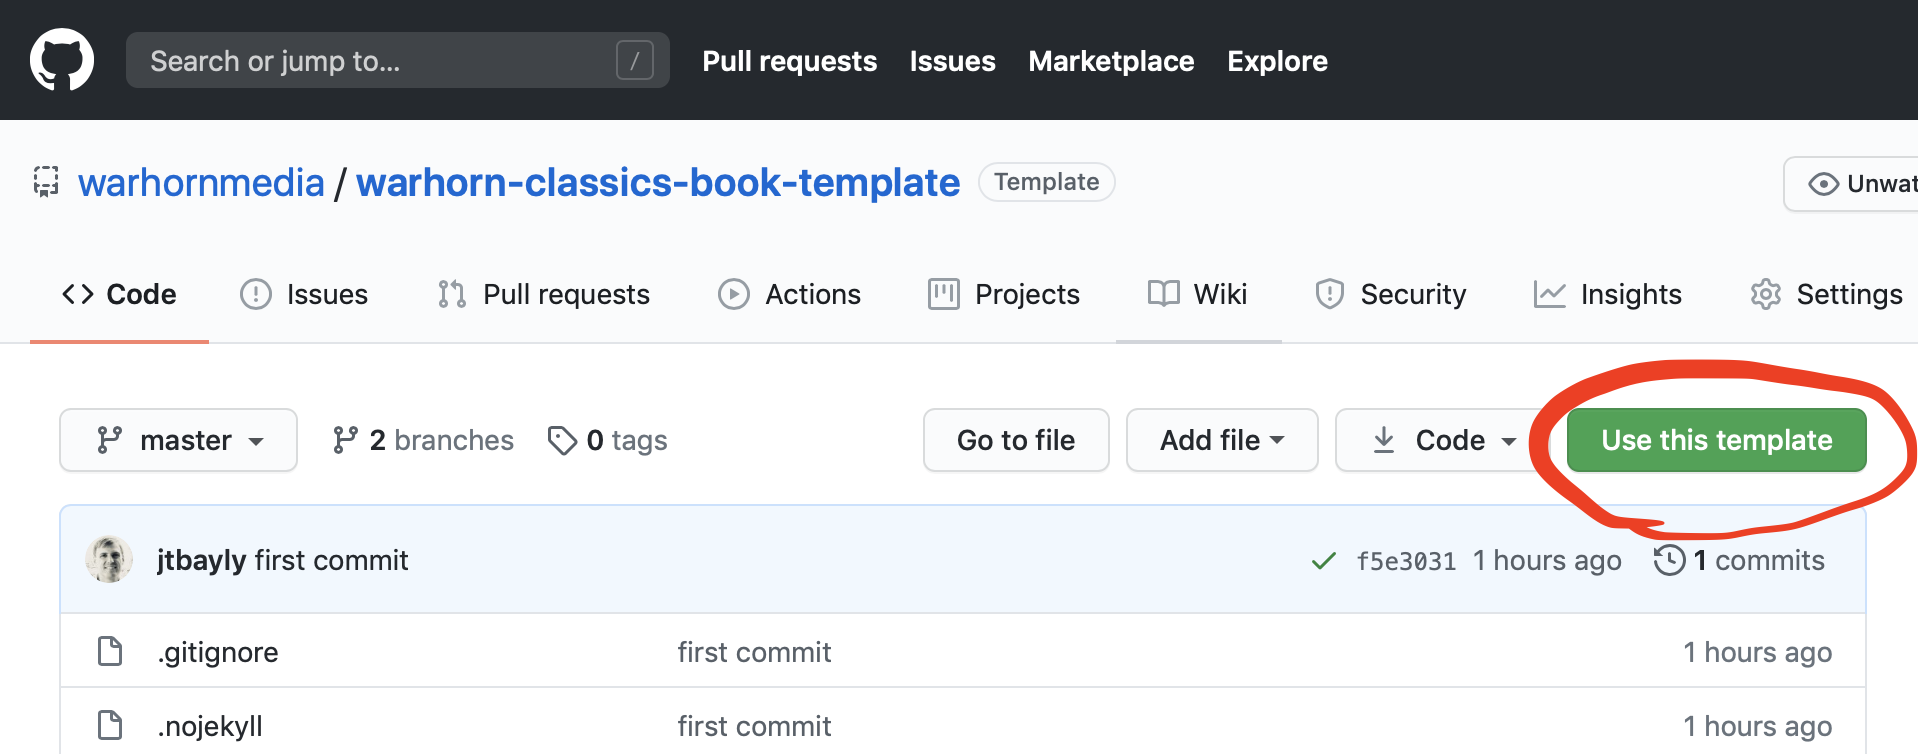
\includegraphics[width=0.65\linewidth]{images/screenshot1} \end{center}

\begin{enumerate}
\def\labelenumi{\arabic{enumi}.}
\setcounter{enumi}{1}
\tightlist
\item
  Change the owner to warhornmedia. Enter a repository name using the format ``authorlastname-short-book-title''. Set the repository to public. And include all branches. Then click ``Create repository from template''
\end{enumerate}

\begin{center}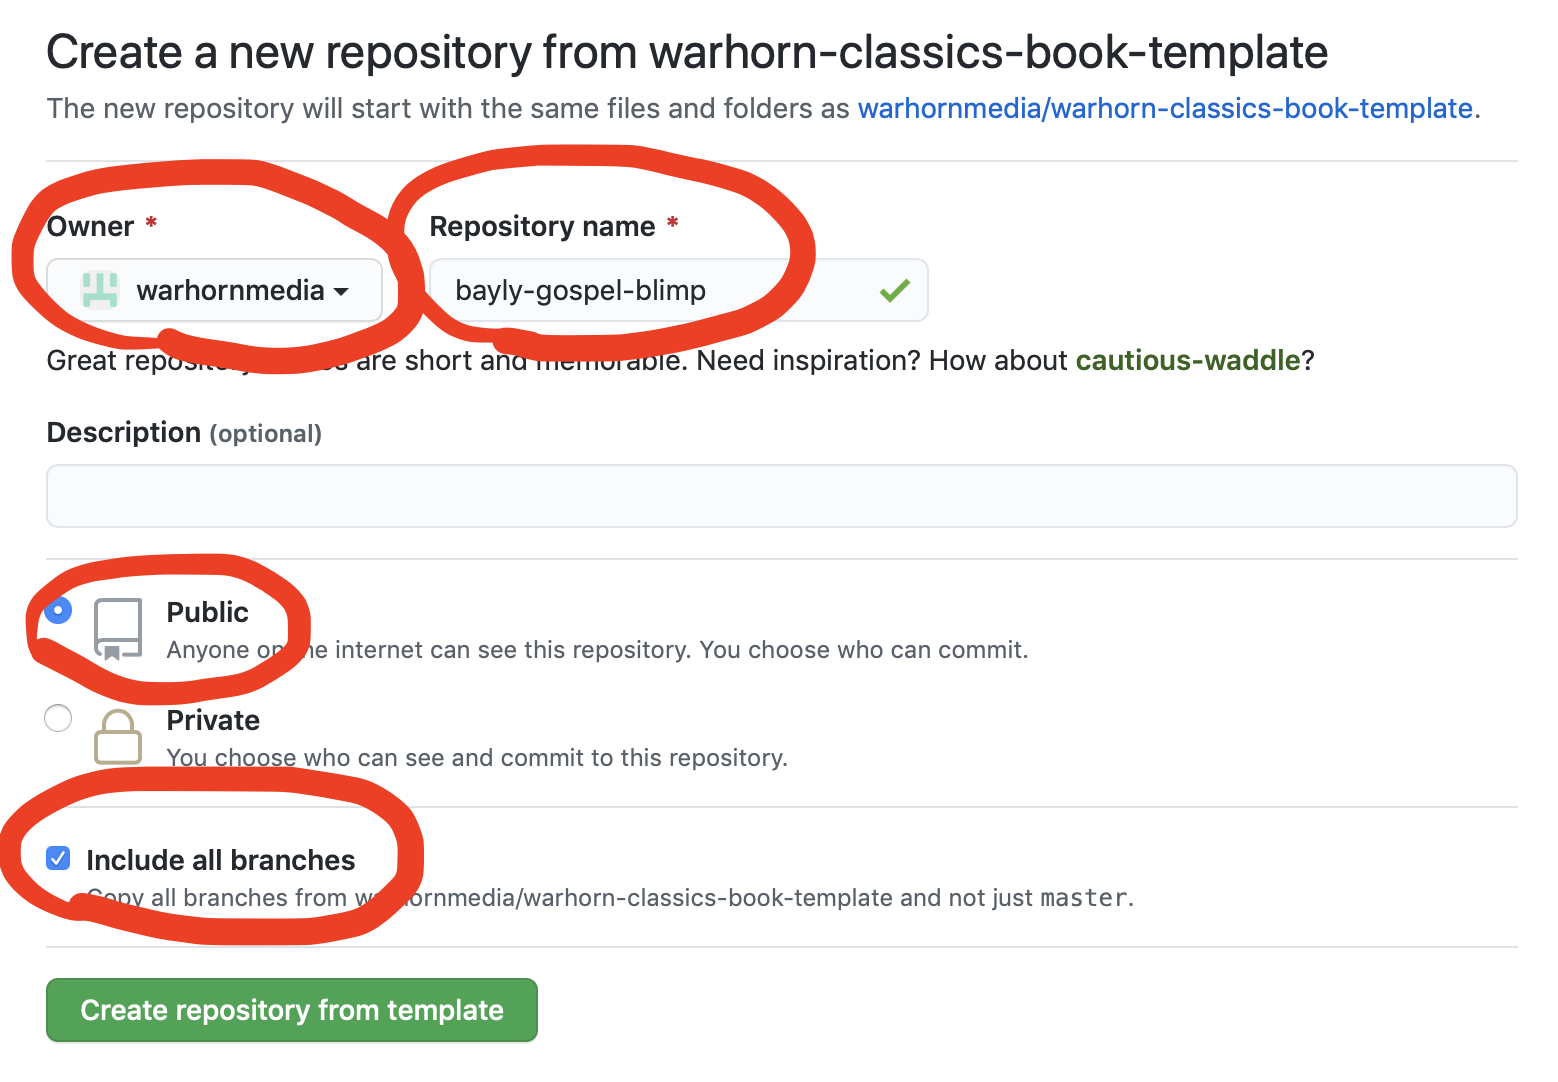
\includegraphics[width=0.65\linewidth]{images/screenshot2} \end{center}

\begin{enumerate}
\def\labelenumi{\arabic{enumi}.}
\setcounter{enumi}{2}
\item
  Clone the new repo to your computer and navigate into its folder in Terminal. Then run the following command locally, answering `yes' to both questions.\footnote{\href{https://docs.github.com/en/free-pro-team@latest/github/authenticating-to-github/creating-a-personal-access-token}{Here are instructions} for creating a Github Personal Access Token if you don't have one yet. (Check the ``repo'' box under ``scopes'' to give the necessary permissions.)

    Also, if you don't have \href{https://github.com/travis-ci/travis.rb\#installation}{travis} installed on your computer yet, you can install it with this command:

\begin{Verbatim}
  brew install travis
\end{Verbatim}

    If you don't have \href{https://brew.sh}{brew} installed yet\ldots{} prepare yourself for some waiting. You can install it with this command:

\begin{Verbatim}
  /bin/bash -c "$(curl -fsSL https://raw.githubusercontent.com/Homebrew/install/master/install.sh)"
\end{Verbatim}
  }

\begin{verbatim}
travis encrypt GITHUB_PAT=yourTokenGoesHere --com --add -x
\end{verbatim}
\end{enumerate}

\emph{Congrats!} You now have a new book that will rebuild automatically any time you push changes to github.

For more in-depth instructions on setting up your new book, as well as important information on how to code the book, check out the \href{https://warhornmedia.github.io/style-guide}{style guide}.

\end{document}
